\documentclass[11pt]{article}
\usepackage{etex}
\usepackage{amssymb}
\usepackage[margin=.8in]{geometry}
\usepackage[table]{xcolor}
\usepackage{amsmath,graphicx}
\usepackage{algorithm}
\usepackage{algorithmicx}
\usepackage{algpseudocode}
\usepackage{alphalph}
\usepackage{listings}
\usepackage{float}
\usepackage{caption}
\usepackage{amsmath}
\usepackage{subcaption}
\usepackage{tabularx}
\usepackage{framed}
\usepackage{tabu}
\usepackage{booktabs}
\usepackage{tikz}
\usepackage[stable]{footmisc}
\usepackage{titlesec}
\usepackage{setspace}
 \usepackage{alltt} 
\usepackage{hyperref}
\usepackage{pgfplots}
\definecolor{shadecolor}{rgb}{0.82,0.82,0.82}




\newcommand{\bt}[1]{\textbf{#1}}    
   
  \begin{document}
  \title{CS691CL - Computational Linguistics: Syntax and Semantics \\ Final Project Report \\ \vspace{1cm} \emph{Document Similarity Measures \\ Utilizing Syntactics and Semantics \\ as well as Embeddings}}
  \author{Nicholas Monath,  Klim Zaporojets, Niklas Shulze}
  \maketitle
  
  
  
\section{Introduction}

There is no shortage of online databases of documents containing valuable information, but there is a need for more tools to organize this data to provide users a more accessible interface than a standard keyword search. Providing solutions to this problem of information overload has been the focus of years of research in information retrieval, natural language processing and machine learning in general. In particular, much work has been done on defining document similarity measures, which determine the relatedness of two documents based on their text content. Typical approaches to this problem are based in word usage statistics and are not able to capture the essence of a text, as the syntactic and semantic relationships of the words are disregarded. In this project, we will make use of dependency parsing and automatic semantic role labeling to extract syntactically and semantically related phrases from text. Using these phrases, we hope to create a more robust document representation and similarity measure than the traditional approaches. 

We also apply our proposed document similarity measure to the problem of identifying relatedness between scientific research papers. The similarity of scientific research papers is a less studied problem than document similarity in general and a robust measure is in high demand \cite{Hurtado2013}. Such a measure would be useful in both research paper recommender systems and search engines. 

The rest of this document is organized as follows: a review of related work done in this field; a description of our document representations and proposed similarity measures; experiments and results; and a conclusion highlighting future work.

\section{Related Work} \label{sec:RelatedWork}

Document similarity is a much studied problem in the field of information retrieval with a wide range of applications, such as document classification and clustering, searching in large unorganized datasets, and recommendation systems. The problem of document similarity extends beyond the measurement of relatedness of \emph{unstructured} documents containing only text to \emph{structured} documents, which contain hyperlinks and other annotations \cite{Manning2008}. 

The most common approach to unstructured text document similarity is a vector space, statistics based method known as the  \emph{bag-of-words} approach. Work in \cite{Huang2008} shows the effectiveness of this simple representation on a number of datasets in the problem of document clustering. Another common technique is the representation of documents with a \emph{language model}. First presented in \cite{Ponte1998}, language models make the assumption that the collection of individual terms in a document is a sample from a probability distribution. This approach is particularly useful in unsupervised document clustering.  Language models are often made more robust by adding additional information such as underlying topic labels obtained algorithms such as \emph{Latent Dirichlet Allocation} (LDA) or \emph{probabilistic latent semantic analysis}.  These models have been shown to be effective in document retrieval and categorization by \cite{Hofmann2000}. 

In these traditional approaches, the syntactic and semantic relationships of words and phrases in the text are ignored. The models are based on statistical information on the frequency of the occurrence of word sequences or $n$-grams. Often unigrams (i.e. $n=1$) are used and so the measure is the frequency of the occurrence of single words. Bigrams (two-word sequences) and trigrams (three-word sequences) are also commonly used. Intuitively, the substitution of \emph{n-grams} with syntactically related groups of words is a logically sound choice. Often, \emph{n-grams} are disparate sequences of terms, while syntactically related groups of words can provide a more robust feature that preserves the semantic meaning of phrases. Initial work was done on this in the late 1990s, such as \cite{Furnkranz1998}, \cite{Dumais1998}. The recent works of \cite{Nastase2007} and \cite{Koster2009}, show the method can have significant benefits over the traditional \emph{n-gram} approach. Nastase et al in \cite{Nastase2007} use syntactically related pairs of words obtained using a dependency parser as the base elements in a vector-based bag-of-words approach to perform the task of supervised text classification on the Reuters-21578 dataset. They also experiment with a combination of using the syntactically related pairs and unigrams both with and without syntactic labels. Koster et al in \cite{Koster2009} use a similar method of combining syntactically related triples obtained with a dependency parser with unigrams in a vector based model to perform the task of patent document classification.

The most recent work related to document similarity of scientific papers can be found in \cite{Hurtado2011} and \cite{Hurtado2013}, it uses a unigram based language model to represent the documents. The model treats the text as \emph{semi-structured}, taking advantage of the additional features of the keywords of the paper, authors' names, and the name of the journal in which the paper appears.

Our work separates itself from these previous studies in that we propose to use syntactically and semantically related sequences of words extracted from the text, using not only dependency parsing, but also automatic predicate argument structure parsing. We also provide a more unified approach to the handling of dependency pairs than \cite{Nastase2007} and \cite{Koster2009}. Additionally, we apply the use of the dependency and predicate argument features to the problems of document clustering and retrieval. 

\section{Document Representations}


\subsection{Document Preprocessing}

In order to extract dependency pair and predicate argument structures from documents for use in a feature structure, we must run documents through a parsing algorithm. The parser we used in \emph{ClearNLP}. We set the parsing mode to be \emph{Semantic Role Labeling}, which produces not only an SRL of the text, but also the dependency structure. The parser also provides additional information about each word it the text: the lemmatized form, part of speech tag, dependency label, semantic role label, and other features. 

\subsection{Bag of ``Units'' Document Representation}

In this work we extend the typical vector space model of a bag of words feature representation to include rich units than single words, namely dependency (head-modifier) pairs, and predicate argument structures. By \emph{units} or \emph{base units} we are referring to the terms whose presence/absence in a document determine the values of the feature vector of the document, its document representation. In this way, each unit corresponds to an entry in the feature vector of a document. The value of that vector can be binary, which means the values of the feature vector are 0 or 1 depending on whether or not a unit appears in the document. It  also can be tf-idf, in which the values of the feature vector are the term-frequency-inverse-document-frequency of a unit. In this project, we used the augmented tf-idf value presented \cite{Polettini2004}.

We experiment with three different units: words, dependency pairs, and predicate/arguments. In the following sections, we present the details of how these units are defined in our system.

\subsection{Feature Settings}

There are a few feature settings which apply to all three of the units. These feature settings determine the form of units that appear in the feature definition. 

\begin{itemize}
 \item \textbf{Lemmatization}: Determines if the lemmatized or un-lemmatized form of the word is used
 \item \textbf{Case Sensitivity}: Determines if a case sensitive version of the word is used
 \item \textbf{Part of Speech Tags}: Determines if part of speech tags are appended to words
 \end{itemize}
 
 
\subsection{Word Units}

We define an object structure representing a single \emph{word} to have the attributes of the \emph{word form} that appears in the document, the \emph{lemmatized form} of the word, and the \emph{part of speech tag} of the word. Equivalence between words is defined through the feature settings. Equivalence is what determines how features are extracted from a document, e.g. suppose we had a feature definition with two words $\{a,b\}$ and are using a binary representation. When extracting a feature from a document, we check each word $w$ in the document, if $w$ is equivalent to $a$ or $b$, then we set the correspond bit in the feature vector to be true. 

If lemmatization is used with part of speech tags, two words are considered equivalent if the character string of their lemmas are the same as well as their part of speech tags. If lemmatization is used without part of speech tags, equivalence is solely determined by the character strings of their lemmas.  If lemmatization is not used then equivalence between words is determined by the character strings of the form the words appear in in the document. This equivalence is also determined by part of speech tags if they are used. Additionally, the case sensitivity option determines if capitalization in the character strings of the word forms effects equivalence. 

\subsubsection{Removing Stop Words}

Rather than using a finite list of stop words, we removed stop words based on the part of speech tags of words. Any words with part of speech tags other than the following are removed:

\begin{figure}[H]
\begin{shaded} \tt
\begin{verbatim}
"JJ", "JJR", "JJS", "NN", "NNS", "NNP", "NNPS", "RR", "RBR", "RBS", "VB", "VBD", 
"VBG", "VBN", "VBP", "VBZ"
\end{verbatim}
\end{shaded}
\caption{Set of Part of Speech Tags of Words Used in the Feature Definition}
\label{fig:KeeperPOS}
\end{figure}

In our future experiments we will experiment with using a finite list of stop words as opposed to this criteria.

\subsection{Dependency Pair Representation}

We define an object structure representing a head-modifier dependency pair to be an ordered tuple of \emph{words} with the structured defined above. The first word in the tuple is the $head$ of the dependency pair, and the second word in the tuple is the modifier of the dependency pair.  Equivalence between dependency pairs is important for the same reason equivalence is important in word units. A dependency pair $dp_1$ is said to be equivalent to another dependency pair $dp_2$ if an only if the word unit which is the head of $dp_1$ is equivalent to the word unit which is the head of $dp_2$ and the word unit which is the modifier of $dp_1$ is equivalent to the word unit which is the modifier of $dp_2$. The additional feature of \textbf{dependency labels} can be used in the representation of dependency pairs. If used, this adds an additional component to the definition of equivalence between dependency pairs, which is that the dependency labels in the pairs must also be the same.

\subsubsection{Removing Stopwords}

The optimal approach to removing stop words from dependency pairs is not entirely clear. We chose the following approach, which we felt was the most logical. We are open to any and all suggestions in how to improve this approach or if other approaches should be taken. 

A dependency pair is removed from the feature if \emph{either the head or modifier or both} have a part of speech tag that is not in the set of part speech tags shown Figure \ref{fig:KeeperPOS}.

\subsubsection{Discovering Dependency Pairs from Parsed File} \label{sec:Discover}


Given the input document:

\begin{shaded} \tt
\begin{verbatim}
My sister thought John Updike's writing was offensive. Mary disagreed.
\end{verbatim}
\end{shaded}

The parsed file is:

\begin{shaded} \tt
\footnotesize
\begin{tabular}{cccccccc}
1 &	My &	my &	PRP\$ &	 \_	& 2	 & poss	 &\_ \\
2 &	sister &	sister &	NN &	\_ &	3 &	nsubj &	3:A0 \\
3 &	thought &	think &	VBD	pb=think.01 &	0 &	root	\_ \\
4 &	John &	john	 &NNP &	\_ &	5 &	nn &	 \_ \\
5 &	Updike &	updike &	 NNP &	\_ &	7 &	poss & \_ \\
6 &	's &	's &	POS	 &\_ &	5 &	possessive &	\_ \\
7 &	writing &	writing &	NN &	\_ &	8 &	nsubj &	8:A1=PPT \\
8 &	was &	be &	VBD	pb=be.01 &	3 &	 ccomp &	3:A1=PPT \\
9 &	offensive &	offensive &	JJ & \_	& 8 &	acomp &	8:A2=PRD \\
10 & 	. & 	. &	. &	\_ &	3 &	punct &	\_ \\

1 &	Mary &	Mary &	PRP	 & \_	 & 2	 & nsubj &	2:A0=PAG \\
2 &	disagreed &	disagree &	VBD	 & pb=disagree.01 & 	0 & 	root	 & \_ \\
3 &	. &	. &	. &	\_ &	2 &	punct &	\_ \\
\end{tabular}
\end{shaded}

The dependency pairs are extracted making use of the intra-sentence word ID numbers (first column) and the corresponding dependency information (fifth column).


\subsection{Predicate Argument Units}

The predicate argument structures extracted from the documents using the semantic role labeler of the parser provide the addition of two units to the feature, predicate units and arguments units. Since we never include one without the other, we refer to them as a group in this report. An additional feature option comes with these units, which is argument labels. If argument labels are used the predicate unit is labeled as a \emph{predicate} and the argument units are labeled with their respective \emph{argument labels} (e.g. A0, AM-TMP etc). Two predicate units are said to be equivalent if the words of the predicate are equivalent and if the additional argument labels are used, if they both have the label \emph{predicate}. Argument units consist of an ordered (in the order they appear in the text) list of words. Two argument units are considered equivalent if  each word in their lists is equivalent and if 
the additional argument labels are used, if they both have the same argument label. 

\subsubsection{Removing Stop Words}

As in the dependency pairs, there are multiple procedures for removing stop words in these units that could be used. The way we removed stop words was by removing any words from the list of words of an argument which do not have a part of speech tag that is in the set in Figure \ref{fig:KeeperPOS}. An argument is removed entirely if the removal of stop words resulted in it having an empty list of words. A relation is removed it the removal of stop words resulted in it having no arguments. 

\subsubsection{Discovering Predicate Argument Structure From Parsed Files} 

In the ClearNLP output file shown in Section \ref{sec:Discover}, we see that we can find the predicate argument structure of each sentence by using the values in the eighth column. The numbers correspond to the predicate associated with the word and the argument label for the argument is provided. Note how only the head word of each argument is labeled. We then follow the dependency paths to discover the entire argument. 

\section{Alternative Document Representations}

\subsection{Embeddings KD Tree}

We define an additional document representation which will be used in the retrieval experiment. In this model, a document is represented as the KD tree of the embeddings of all of the words that appear in the document. The distance between documents $D_1$ and $D_2$ with this representation is defined as 0.5 times the average distance of between each embedding in $D_1$  and the closest embedding $D_2$ plus 0.5 times the average distance of between each embedding in $D_2$  and the closest embedding $D_1$


\section{Experiments}

\definecolor{tableShade}{gray}{0.9}
\colorlet{tableheadcolor}{black!90} % Table header colour = 25% gray
\newcommand{\headcol}{\rowcolor{tableheadcolor}} %
\rowcolors{3}{tableShade}{white}  %% start alternating shades from 3rd row



Due to limited computational resources and the immense size of the datasets we were not able to evaluate how our methods did compared to the state of the art. Instead, we ran a set of experiments comparing our methods to a baseline unigram bag of words approach. These experiments will provide insight into whether or not the additional features extracted using dependency pairs and predicate argument structures is beneficial to a document similarity measure. 

In these experiments, we compared the performance of four of our feature representations. We performed the experiments on the feature definitions with each of the following combinations of units:

\begin{itemize}
\item Words
\item Words and Dependency Pairs 
\item Words and Predicate Argument Structures
\item Words, Dependency Pairs, and Predicate Argument Structures
\end{itemize}

We experimented with both a binary and a tf-idf valued feature vectors. Due to computational constraints, we used only the lemmatized version of words and did not use part of speech, dependency labels, nor argument labels. Features that appeared in only one document where removed from the feature definition.


\section{Document Clustering} \label{sec:DocumentClusterting}

\subsection{General Setup}

The problem of \bt{document clustering} is defined as the automatic organization of documents into logical groups based on latent features. For evaluation purposes, we use documents that are already divided into classes. We then use a clustering algorithm to see how well the clusters represent the true classes of the documents. 

Formally, the experimental set up is as follows. Given a collection of documents $D_1$, $D_2$, $\dots$ $D_N$,  which have been preprocessed in the method described above. The first step of the experiment is to define a feature for the documents, i.e. union of the set of all units (words, dependency pairs, predicate/argument structures), which appear in at least one document in the collection. We then extract a feature vector from each of these documents to produce the set of features for the documents $X_1$, $X_2$, $\dots$ $X_N$. Each document has an associated class label $y_1$, $y_2$, $\dots$, $y_N$, which will be used to in evaluating the performance of the clustering algorithm.

In these, experiments we clustered the document features $X_1$, $X_2$, $\dots$ $X_N$ using the $k$-means clustering algorithm with $k$ being the number of unique class labels for the documents. For a distance function, we used the Cosine Similarity in that we normalized $X_1$, $X_2$, $\dots$ $X_N$  to unit length and used a Euclidean distance measure. The output of the clustering algorithm is a cluster id label for each of the $N$ documents, which we will refer to as $C_1$, $C_2$, $\dots$, $C_N$. 


\subsection{Evaluation Measures}

Following the experiments in \cite{Huang2008} and \cite{Hofmann2000}, we evaluated the clustering of the documents with the measures of purity, normalized mutual information, and the adjusted Rand index. The definitions of these metrics are from \cite{Manning2008}.

\subsubsection{Purity}

Purity is a measure of cluster quality, that is how well the classes are defined into clusters. If we refer to $Y$ as the set of unique class labels in the data set, and refer to $W_i$ as the class labels of the documents in the $i^{th}$ cluster. The purity is defined as follows:

\begin{equation}
{\text{Purity}}(W_{1:K}, Y) = \frac{1}{N} \left ( \sum_{n=1}^N \max_{y \in Y} \left (\sum_{w \in W_n} [w = y] \right ) \right )
\end{equation} 

where $[w=y]$ is the indicator function--it evaluates to 1 if $w$ is equal to $y$ and evaluates to 0 otherwise. 

\subsubsection{Normalized Mutual Information}

The normalized mutual information between the cluster indexes $C_1$, $C_2$, $\dots$, $C_N$ and the class labels  $Y_1$, $Y_2$, $\dots$, $Y_N$ is measured. This is defined as:

\begin{equation}
\text{NormalizedMutualInformation}(C_{1:N}, Y_{1:N}) = \frac{I(C_{1:N}, Y_{1:N}) }{H(C_{1:N}) + H(Y_{1:N}) }
\end{equation}

Where $I$ is the mutual information:

\begin{align}
I(C_{1:N}, Y_{1:N}) &= \sum_i \sum_j {P(C_i, Y_j)} \frac{P(C_i, Y_j)}{P(C_i)P(Y_j)} \\
\end{align}

and the entropy $H$ is:

\begin{align}
H(C_{1:N}) = - \sum_i P(C_i) \log P(C_i) \\
H(Y_{1:N}) = - \sum_i P(Y_i) \log P(Y_i) \\
\end{align}

and the probability distributions are their maximum likelihood estimates. 

\subsubsection{Adjusted Rand Index}

The adjusted Rand index is a version of the Rand index that is adjusted for the chance grouping of elements. In general the Rand index evaluates the similarity between $C_{1:N}$ and $Y_{1:N}$. For the sake of time, we will not present the full definition of the Adjusted Rand index here, but refer readers to \cite{Yeung2001} for its definition.

\subsection{Reuters-21578}

We selected a portion of the test cases of the Mod-Apte split of the Reuters-21578 to use in a clustering experiment. We selected those documents from the top 8 most frequently appearing classes and that only belonged to one class. This selection was inspired by the experiments in \cite{Nastase2007} and \cite{Hofmann2000}. The distribution of documents in the data set can be see in figure \ref{fig:ReutersClassDist}. The results for each of our feature vectors shown in Table \ref{tbl:ReutersClusteringResults}. 

\begin{figure}[H]
\centering
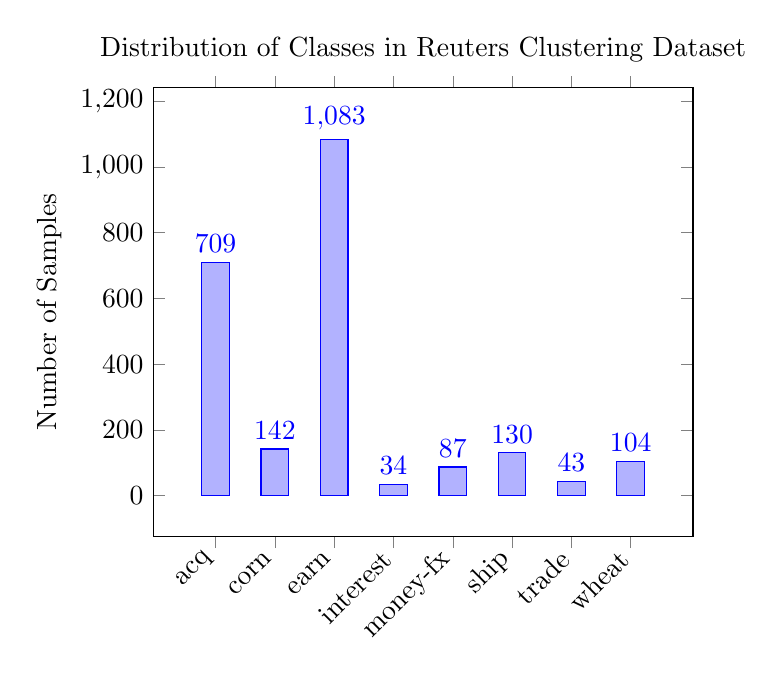
\begin{tikzpicture}
  \begin{axis}[
    ybar,
    enlargelimits=0.15,
    legend style={at={(0.5,-0.2)},
      anchor=north,legend columns=-1},
    ylabel={Number of Samples},
    symbolic x coords={acq,corn,earn,interest,money-fx,ship,trade,wheat},
    xtick=data,
    nodes near coords,
    nodes near coords align={vertical},
    x tick label style={rotate=45,anchor=east},
    title=Distribution of Classes in Reuters Clustering Dataset
    ]
    \addplot coordinates {(acq,709) (corn,142)
        (earn,1083) (interest,34) (money-fx,87) (ship, 130) (trade, 43) (wheat, 104)};
  \end{axis}
  \end{tikzpicture}
  \caption{Class Distribution}
  \label{fig:ReutersClassDist}

\end{figure}

\begin{table}[H]
\caption{Reuters Clustering Results}
\label{tbl:ReutersClusteringResults}
\begin{tabular}{|c|c|c|c|c|}
\hline
\headcol \color{white} Feature Type & \color{white} Value Type & \color{white} Purity & \color{white} Normalized Mutual  & \color{white} Adjusted Rand  \\
 \headcol & & &  \color{white} Information & \color{white}  Index \\
\hline
Words & Binary & 0.72727 & 0.44211 &  0.20537  \\
Words & tf-idf &  0.761149  & 0.50932 & 0.33894\\
Words \& Dep. Pairs & Binary & 0.711835 & 0.42011 & 0.15659 \\
Words \& Dep. Pairs & tf-idf & 0.699828 & 0.34044 & 0.05001 \\
Words \& Pred. Arg. & Binary & 0.761149 & 0.490585 & 0.32799 \\
Words \& Pred. Arg.  & tf-idf & \textbf{0.786878} & \textbf{0.5485359} & \textbf{0.37705} \\
Words, Dep. Pairs, \& Pred. Arg. & Binary & 0.729845 & 0.442120 & 0.22446 \\
Words, Dep. Pairs, \& Pred. Arg.& tf-idf & 0.75 & 0.491923 & 0.30966 \\
\hline
\end{tabular}
\end{table}


\subsection{Brown Corpus}

The next clustering experiment we ran was on the Brown Corpus. We ran the same document clustering experiment described earlier on the 500 document corpus. The Brown Corpus has a slightly more even class distribution than the Reuters Corpus:

\pgfplotsset{width=12cm}
\begin{figure}[H]
\label{fig:BrownClassDist}
\centering
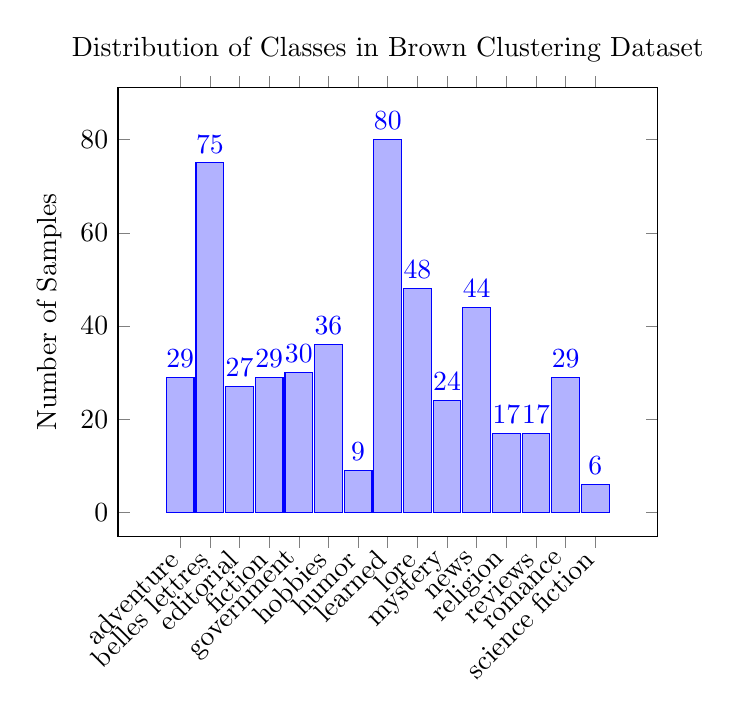
\begin{tikzpicture}
  \begin{axis}[
    ybar,
    enlargelimits=0.15,
    legend style={at={(0.5,-0.2)},
      anchor=north,legend columns=-1},
    ylabel={Number of Samples},
    symbolic x coords={adventure,belles lettres,editorial,fiction,government,hobbies,humor,learned,lore,mystery,news,religion,reviews,romance,science fiction},
    xtick=data,
    nodes near coords,
    nodes near coords align={vertical},
    x tick label style={rotate=45,anchor=east},
    title=Distribution of Classes in Brown Clustering Dataset
    ]
    \addplot coordinates {(adventure, 29) (belles lettres, 75) (editorial, 27) (fiction, 29) (government, 30) (hobbies, 36) (humor, 9) (learned, 80) (lore, 48) (mystery, 24) (news, 44) (religion, 17) (reviews, 17) (romance, 29) (science fiction, 6)};
  \end{axis}
  \end{tikzpicture}
\end{figure}

\begin{table}[H]
\caption{Brown Corpus Clustering Results}
\label{tbl:BrownClusteringResults}
\begin{tabular}{|c|c|c|c|c|}
\hline
\headcol \color{white} Feature Type & \color{white} Value Type & \color{white} Purity & \color{white} Normalized Mutual  & \color{white} Adjusted Rand  \\
 \headcol & & &  \color{white} Information & \color{white}  Index \\
\hline
Words & Binary & 0.384 & 0.35450 &  0.13015  \\
Words & tf-idf &  0.39  & 0.32450 & 0.12138 \\
Words \& Dep. Pairs & Binary & 0.388 & \textbf{0.3760} & 0.13765 \\
Words \& Dep. Pairs & tf-idf & 0.388 & 0.32795 & 0.12595 \\
Words \& Pred. Arg. & Binary & 0.406 & 0.37245 & \textbf{0.17063} \\
Words \& Pred. Arg.  & tf-idf & 0.374 & 0.3249 & 0.12786\\
Words, Dep. Pairs, \& Pred. Arg. & Binary & 0.368 & 0.32627 & 0.1205 \\
Words, Dep. Pairs, \& Pred. Arg.& tf-idf & \textbf{0.414} & 0.34935 & 0.1424 \\
\hline
\end{tabular}
\end{table}


\subsection{Scientific Paper Dataset} \label{sec:ScientificPaperClustering}

We collected a small dataset of the abstracts, titles, and authors \footnote{There are no meta-data tags of in the documents, only text. This experimental setup was designed to partially mimic the experiments in \cite{Hurtado2013}} of the papers that we read in this courses. Each paper was given the class label of the unit it was a part of--unit being ``Tree Adjoining Grammar'' or ``Ontology and Taxonomy''. The name of each paper and the  class label assigned is shown in Table \ref{tbl:ScientificPaperClassListing}. While this is a relatively small dataset of just 22 documents, the domain was significantly different enough from the previous two datasets to be worthy of experimentation. The results are shown in Table \ref{tbl:ScientificPaperClusteringResults}

Note that for a small number of these papers, there was no abstract. In these cases, if the introduction was brief, the introduction was used in lieu of the abstraction, otherwise the document was not a part of the dataset. Also note that the conversion from PDF to plain text was done manually.


\begin{table}[H]
\centering
\footnotesize
\caption{Class Assignments in Scientific Paper Dataset}
\label{tbl:ScientificPaperClassListing}
\begin{tabular}{|c|c|}
\headcol \color{white} Paper Title & \color{white} Class Name \\
\hline
Penn Treebank Overview & Phrase Structure Grammar \\
Government \& Binding Theory Introduction & Phrase Structure Grammar \\ 
Introduction to Prop Bank & Predicate Argument Structure \\ 
On the Semantic Content of the Notion of Thematic Role & Predicate Argument Structure \\
Tree Adjoining Grammars & Tree Adjoining Grammars \\
Domains of Locality & Tree Adjoining Grammars \\
Synchronous Tree Adjoining Grammars & Tree Adjoining Grammars \\
Supertagging: An Approach to Almost Parsing & Tree Adjoining Grammars \\
Introduction to WordNet: An On-line Lexical Database & WordNet \\
Nouns in WordNet: A Lexical Inheritance System & WordNet \\
Adjectives in WordNet & WordNet \\
English Verbs as a Semantic Net & WordNet \\
Design and Implementation of WordNet Lexical Database and Searching Software & WordNet \\
Never Ending Language Learner & Ontology and Taxonomy \\
Which Noun Phrases Denote Which Concepts & Ontology and Taxonomy \\
Combinatory Categorial Grammar by Steedman and Baldridge & Combinatory Categorial Grammar \\
Equivalence of Four Extensions of Context Free Grammars & Combinatory Categorial Grammar \\
Vector Space Semantic Parsing & Combinatory Categorial Grammar \\
FrameNet II & Frame Semantics in FrameNet \\
A Frames Approach to Semantic Analysis & Frame Semantics in FrameNet \\
Learning to Map Sentence to Logical Form & Distributional Semantics \\
Relation Extraction with Matrix Factorization and Universal Schema & Distributional Semantics \\
\hline
\end{tabular}
\end{table}



%TODO Insert the Correct values
\begin{table}[H]
\centering
\caption{Scientific Paper Clustering Results}
\label{tbl:ScientificPaperClusteringResults}
\begin{tabular}{|c|c|c|c|c|}
\hline
\headcol \color{white} Feature Type & \color{white} Value Type & \color{white} Purity & \color{white} Normalized Mutual  & \color{white} Adjusted Rand  \\
 \headcol & & &  \color{white} Information & \color{white}  Index \\
\hline
Words & Binary & 0.69565 & 0.73913 &  0.40844 \\
Words & tf-idf &  0.69565  & 0.74719 & 0.33894\\
Words \& Dep. Pairs & Binary & \textbf{0.782608} & 0.79312 & 0.52854 \\
Words \& Dep. Pairs & tf-idf & 0.69565 & 0.763719 & 0.515285 \\
Words \& Pred. Arg. & Binary & 0.69565 & 0.760097 & 0.518171 \\
Words \& Pred. Arg.  & tf-idf & {0.69565} & {0.73288} & {0.38731} \\
Words, Dep. Pairs, \& Pred. Arg. & Binary & \textbf{0.782608} & \textbf{0.80828} & \textbf{0.53292} \\
Words, Dep. Pairs, \& Pred. Arg.& tf-idf & 0.69565 & 0.72555 & 0.44924 \\
\hline
\end{tabular}
\end{table}

\subsection{Analysis}

These experimental results showed that including richer features (dependency pairs and predicate argument structures) improves document clustering results. It is seen that the Reuters dataset is slightly easier to cluster than the Brown corpus, most likely because the classes are more distinct. We also see that in the Reuters and Brown experiments, the Words and Predicate Argument Structures feature did the best, while in the scientific paper experiment the words and dependency pairs feature performed the best. This is likely because the predicates in the scientific papers are less distinctive than in the other two works. 



\section{Document Classification}

\subsection{General Problem Description and Evaluation Criteria}

In general the problem of document classification is defined as: given set of training samples, pairs of documents and associated class labels: $(D_1, Y_1)$, $(D_2, Y_2)$, \dots, $(D_N, Y_N)$, predict the class label for a document $D_{N+1}$ not a part of the training set. From the training documents we first define a feature vector in the same way described in clustering experiment. We then extract features from the training set to get the set of features for all the training documents: $X_1,\ X_2$, $\dots$, $X_N$. We use the same feature definition to extract features from the testing documents. 

The classifier we used in this experiment was an SVM with a Linear Kernel. We used a value of $C=1$. In future experiments we will use a lower value of $C$. We again used Cosine similarity by normalizing the features and using the Euclidean distance.  

The classification task was evaluated on the standard criteria of accuracy, and the average per-class precision and recall scores.

\subsection{NewsGroups Classification Experiment \#1}

The entire Twenty News Groups Corpus consists of about 18 thousand documents, about 11 thousand training and 7 thousand testing. The data set was too large to run our machines and so we selected a smaller portion of the data set to use in our experiments. From the original training and testing sets, we created new sets of the first 200 samples of the 15 most frequently occurring classes. The results from our experiment are shown in Table \ref{tbl:NewsGroupsClassification1}.

%TODO Insert the Correct values
\begin{table}[H]
\centering
\caption{NewsGroups Classification Experiment \#1 Results}
\label{tbl:NewsGroupsClassification1}
\begin{tabular}{|c|c|c|c|c|}
\hline
\headcol \color{white} Feature Type & \color{white} Value Type & \color{white} Accuracy & \color{white} Avg. Precision  & \color{white} Avg. Recall \\
 \headcol & & &  \color{white} Per Class & \color{white}  Per Class \\
\hline
Words & Binary & 0.81033 & 0.809039 &  0.81033  \\
Words & tf-idf &  \textbf{0.852}  & \textbf{0.85082} & \textbf{0.852} \\
Words \& Dep. Pairs & Binary & 0.81266 & 0.811923 & 0.81266 \\
Words \& Dep. Pairs & tf-idf & 0.849 & 0.84849 & 0.849 \\
Words \& Pred. Arg. & Binary & 0.8143 & 0.81348 & 0.8143 \\
Words \& Pred. Arg.  & tf-idf & {0.84933} & {0.84829} & {0.84933} \\
Words, Dep. Pairs, \& Pred. Arg. & Binary & 0.81333 & 0.812843 & 0.81333 \\
Words, Dep. Pairs, \& Pred. Arg.& tf-idf & 0.84766 & 0.847274 & 0.84766 \\
\hline
\end{tabular}
\end{table}

\subsection{NewsGroups Classification Experiment \#2}

As a second classification experiment, we selected the first 100 samples of all of the twenty classes in both the training and testing sets.  The results for this experiment are shown in Table \ref{tbl:NewsGroupsClassification2}.

%TODO Insert the Correct values
\begin{table}[H]
\centering
\caption{NewsGroups Classification Experiment \#2 Results}
\label{tbl:NewsGroupsClassification2}
\begin{tabular}{|c|c|c|c|c|}
\hline
\headcol \color{white} Feature Type & \color{white} Value Type & \color{white} Accuracy & \color{white} Avg. Precision  & \color{white} Avg. Recall \\
 \headcol & & &  \color{white} Per Class & \color{white}  Per Class \\
\hline
Words & Binary & 0.718 & 0.721072 &  0.718  \\
Words & tf-idf &  0.768  & 0.773496 & 0.768\\
Words \& Dep. Pairs & Binary & 0.719 & 0.72428 & 0.719 \\
Words \& Dep. Pairs & tf-idf & \textbf{0.7705} & \textbf{0.77597} & \textbf{0.7705} \\
Words \& Pred. Arg. & Binary & 0.7175 & 0.72105 & 0.7175 \\
Words \& Pred. Arg.  & tf-idf & 0.7685 & 0.77455 & 0.7685\\
Words, Dep. Pairs, \& Pred. Arg. & Binary &  0.717 & 0.721931 &  0.717 \\
Words, Dep. Pairs, \& Pred. Arg.& tf-idf & 0.7705 & 0.77488 & 0.7705 \\
\hline
\end{tabular}
\end{table}

\subsection{Analysis}

In the first experiment, we were not able to out perform the unigram baseline approach. This is likely due to over-fitting during training. We used a far too over-fitting value of $C=1$ in our support vector machine. This mistake will be one of the first that we correct this summer. The second experiment was consistent with our hypothesis that in the presence of small amounts of data our document representation can provide great separation between the classes of documents. Interestingly, in this experiment, the increase in performance came with the addition of only dependency pairs rather than the predicate argument structures. The improvement over the baseline is only about 1.5 points. We will be investigating document classification further in our future work this summer. 


\section{Document Retrieval}

As a final experiment, we ran a simplified version of a document retrieval system. The problem definition is as follows: Given a collection of documents $D_1$, $D_2$, $\dots$, $D_N$, each with a class label $Y_1$, $Y_2$, $\dots$, $Y_N$, query the collection on each document $D_i$ and retrieval the top $K$ documents with lowest Cosine distance. The precision/recall of each retrieval is scored and the average across all queries is reported. The feature vectors representing the documents are defined using the entire corpus. 

\subsection{Scientific Paper Retrieval}

We first ran the retrieval experiment on the Scientific Paper dataset described in Section \ref{sec:ScientificPaperClustering}. In this experiment we retrieved the top $K=5$ closest
documents. This experiment was meant to be a precursor to the work we will do this summer replicating a similar experiment presented in \cite{Hurtado2013}. 

%TODO Insert the Correct values
\begin{table}[H]
\centering
\caption{Scientific Paper Retrieval Results}
\label{tbl:ScientificPaperRetrievalResults}
\begin{tabular}{|c|c|c|c|}
\hline
\headcol \color{white} Feature Type & \color{white} Value Type & \color{white} Avg. Precision  & \color{white} Avg. Recall \\
\hline
Words & tf-idf & 0.423913 &   0.71377  \\
Words \& Dep. Pairs & tf-idf & 0.423913 & 0.71377 \\
Words \& Pred. Arg. & tf-idf & 0.402173  & 0.65579 \\
Words \& Pred. Arg.  & tf-idf &  {0.423913} & {0.713768} \\
Embeddings KD-Tree & - & 0.347826 & 0.565217 \\
\hline
\end{tabular}
\end{table}

\subsection{Brown Corpus Retrieval}

We ran an additional retrieval experiment, in which we selected the first 15 samples of the top 5 most frequently occurring classes in the Brown corpus. We then ran the retrieval experiment with $K=15$. Note that in this case the precision and recall is the same, it is just the percentage of the top 15 documents that were of the same class of the query document. 

\begin{table}[H]
\centering
\caption{Brown Retrieval Results}
\label{tbl:BrownRetrievalResults}
\begin{tabular}{|c|c|c|c|}
\hline
\headcol \color{white} Feature Type & \color{white} Value Type & \color{white} Avg. Precision  & \color{white} Avg. Recall \\
\hline
Words & Binary & 0.460952 &   0.460952  \\
Words \& Dep. Pairs & tf-idf &  0.47047  & 0.47047\\
Words \& Pred. Arg. & tf-idf & 0.463809  & 0.463809 \\
Words, Dep. Pairs, \& Pred. Arg. & tf-idf & \textbf{0.47619} & \textbf{0.47619} \\
Embeddings KD-Tree & - & 0.45523 & 0.45523 \\
\hline
\end{tabular}
\end{table}

\subsection{Analysis}

It's not entirely clear why the additional features of dependency pairs and predicate argument structures do not provide  the same benefit in this retrieval experiment that they did in the other two experiments. It is possible that the experiment size is just too small for the results to be considered meaningful. With more data the feature space will expand and in so doing spread the document's feature vectors farther apart in the space. An interesting follow up experiment would be similar to $K$-nearest neighbor classification, that is to take the training data from one of the data sets, use this data to define a feature, and extract features using this definition from the training documents. Then for evaluation, we query the data set on held out samples (e.g. the testing set of the data set). 



\section{Conclusions and Future Work}

Our experimental results revealed that vector space document similarity measures can be improved by including richer features such as dependency pairs and predicate argument structures. While these experiments were performed on smaller size datasets, they seem to support our hypothesis that these additional features can make vector space models for documents more distinguishable even when the amount of data of is limited. We will continue to work on this project in the summer. One of our first tasks will be to create an additional baseline of a bag of words model using bigrams and trigrams. Next, we will fine tune our code and run it on the full datasets on a machine that is more powerful than our laptops. We will also investigate tuning the hyper-parameters of the classifiers and clustering algorithms. 

Once a more conclusive study of the performance of our system is complete. We will spend time trying to beat the state of the art. We will finish implementing the algorithm of the paper \cite{Nastase2007}, which also made use of dependency information. Additionally, we spend time setting up the experiment done in \cite{Hurtado2013}. This experiment uses scientific abstracts papers from the Web of Science as the data set. We hope to out perform the state of the art on this dataset. 

Finally, we hope to implement portions of the project, which were stated in the proposal but we did not have time to implement. We hope to implement language model document representation that perhaps makes use of LDA. We also hope to further study the Embedding KD Tree document representation, to understand why it does not perform  as well as the vector space models.  


\nocite{*}

\bibliographystyle{plain}
\bibliography{references}
  
  \end{document}